\documentclass{article}

\usepackage{amsmath}
\usepackage{amssymb}
\usepackage{amsfonts}
\usepackage{fullpage}
\usepackage{graphicx}
\usepackage{float}


\makeatletter
\def\moverlay{\mathpalette\mov@rlay}
\def\mov@rlay#1#2{\leavevmode\vtop{%
   \baselineskip\z@skip \lineskiplimit-\maxdimen
   \ialign{\hfil$\m@th#1##$\hfil\cr#2\crcr}}}
\newcommand{\charfusion}[3][\mathord]{
    #1{\ifx#1\mathop\vphantom{#2}\fi
        \mathpalette\mov@rlay{#2\cr#3}
      }
    \ifx#1\mathop\expandafter\displaylimits\fi}
\makeatother

\newcommand{\cupdot}{\charfusion[\mathbin]{\cup}{\cdot}}
\newcommand{\bigcupdot}{\charfusion[\mathop]{\bigcup}{\cdot}}

\title{MA 3231 Homework 1}

\setlength\parindent{0pt}
\begin{document}
\maketitle

\begin{enumerate}

%%%% 1 %%%%
\item 

Let $x_1$ be the number of tons of bands produced, $x_2$ be the number of tons of coils produced, and $z$ be the steel company's profit in dollars.

\begin{align*}
&\max z = 25x_1 + 30x_2 \\
&\text{subject to}\\
&\frac{1}{200}x_1 + \frac{1}{140}x_2 \leq 40 \\
&x_1 \leq 6000 \\
&x_2 \leq 4000 \\
&x_1,x_2 \geq 0
\end{align*}

Band production offers $25\cdot 200 = 5000$ dollars of profit per hour and coil production offers $30 \cdot 140 = 4200$ dollars of profit per hour. To maximize profit first exhaust all allowable band production and then shift to coil production. Obtain 6000 tons of bands using 30 hours of production time and use the remaining 10 hours of production time to obtain 1400 tons of coils. The optimal solution to this problem is \$192,000 of profit when 6000 tons of bands are produced and 1400 tons of coils are produced.

$$
\boxed{z = 192,000 \text{ at } (x_1,x_2) = (6000,1400)}
$$


\newpage
%%%% 2 %%%%
\item 

Define the variables $x_1, \dots , x_9$ and  $z$ as

\begin{align*}
x_1 &: \text{ Number of Ithaca-Newark tickets, Y class} \\
x_2 &: \text{ Number of Ithaca-Newark tickets, B class} \\
x_3 &: \text{ Number of Ithaca-Newark tickets, M class} \\
x_4 &: \text{ Number of Newark-Boston tickets, Y class} \\
x_5 &: \text{ Number of Newark-Boston tickets, B class} \\
x_6 &: \text{ Number of Newark-Boston tickets, M class} \\
x_7 &: \text{ Number of Ithaca-Boston tickets, Y class} \\
x_8 &: \text{ Number of Ithaca-Boston tickets, B class} \\
x_9 &: \text{ Number of Ithaca-Boston tickets, M class} \\
z &: \text{ Ticket revenue in dollars}
\end{align*}

The plane can hold 30 passengers while traveling between Ithaca and Newark. This includes passengers traveling from Ithaca to Newark ($x_1,x_2,x_3$) and passengers traveling from Newark to Boston ($x_7,x_8,x_9$). Similarly the plane can hold 30 passengers while traveling between Newark and Boston. This includes passengers traveling from Newark to Boston ($x_4,x_5,x_6$) and passengers traveling from Ithaca to Boston ($x_7,x_8,x_9$). 

\begin{align*}
&\max z = 300x_1 + 220x_2 + 100x_3 + 160x_4 + 130x_5 + 80x_6 + 360x_7 + 280x_8 + 140x_9 \\
&\text{subject to} \\
&x_1 + x_2 + x_3 + x_7 + x_8 + x_9 \leq 30 \\
&x_4 + x_5 + x_6 + x_7 + x_8 + x_9 \leq 30 \\
&x_1 \leq 4 \\
&x_2 \leq 8 \\
&x_3 \leq 22 \\
&x_4 \leq 8 \\
&x_5 \leq 13 \\
&x_6 \leq 20 \\
&x_7 \leq 3 \\
&x_8 \leq 10 \\
&x_9 \leq 18 \\
&x_1,x_2,x_3,x_4,x_5,x_6,x_7,x_8,x_9 \geq 0
\end{align*}

\newpage
%%%% 3 %%%%
\item 

To convert to standard form the problem must be written so that we maximize the objective function and all constraints (besides the nonnegativity constraints) are written using '$\leq$'. For the objective function, minimizing $z = x_1 - 2x_2 -3x_3$ is equivalent to maximizing $z' = -z = -x_1 + 2x_2 +3x_3$. Then redefine $z:= z'$. The constraint $x_1 - x_2 + x_3 = 2$ is equivalent to the combination of the two constraints $x_1 -x_2 + x_3 \leq 2$ and $x_1 - x_2 + x_3 \geq 2$. Negate the constraint $x_1 - x_2 + x_3 \geq 2$ in order to write this constraint in standard form. 

\begin{align*}
&\max z = -x_1 + 2x_2 + 3x_3 \\
&\text{subject to}\\
&x_1 + 2x_2 + x_3 \leq 14 \\
&-x_1 - 2x_2 - 4x_3 \leq -12 \\
&x_1 - x_2 + x_3 \leq 2 \\
&-x_1 + x_2 - x_3 \leq -2 \\
&-x_3 \leq 3\\
&x_1, x_2, x_3 \geq 0
\end{align*}


\newpage
%%%% 4 %%%%
\item  The first figure shows the boundary lines for each constraint. Since the constraints require that $(x_1,x_2)$ lie underneath each of these lines within the first quadrant, the feasible region is just the area bounded by $3x_1 + 3x_2 \leq 2$. The second figure shows level curves for increasing $z$ values. The value of $z$ is maximized in the feasible region by shifting level curve $z = c$ outward as far as possible while still making sure at least one point on $z=c$ lies within the feasible region. The optimal value of $z$ is 

$$
\boxed{z= 2 \text{ at } (x_1,x_2) = (0,2/3)}
$$ 

\begin{figure}[H]
\centering
  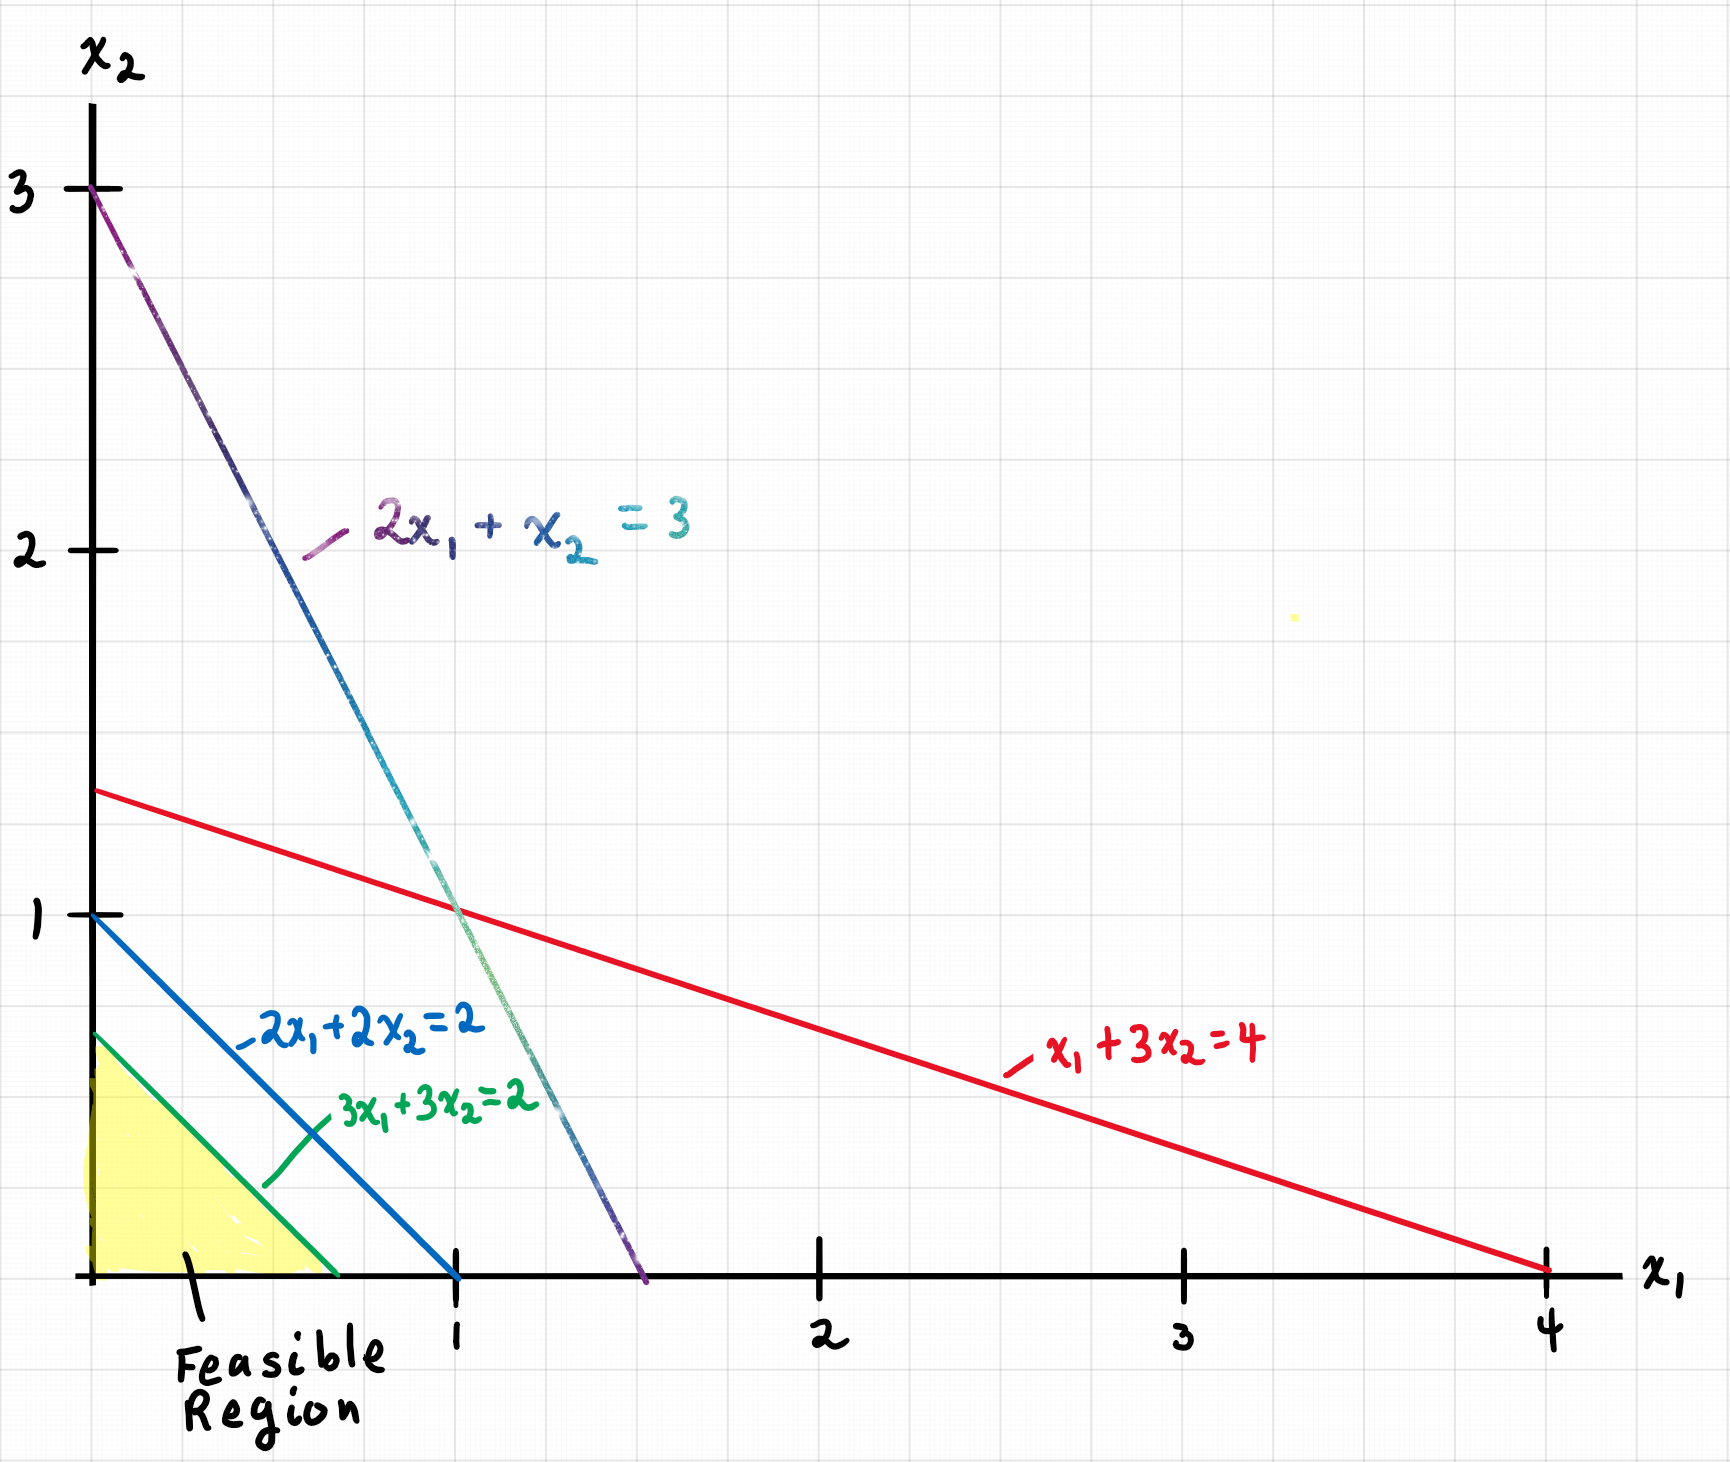
\includegraphics[width=0.65\linewidth]{Capture 1.png}
\end{figure}

\begin{figure}[H]
\centering
  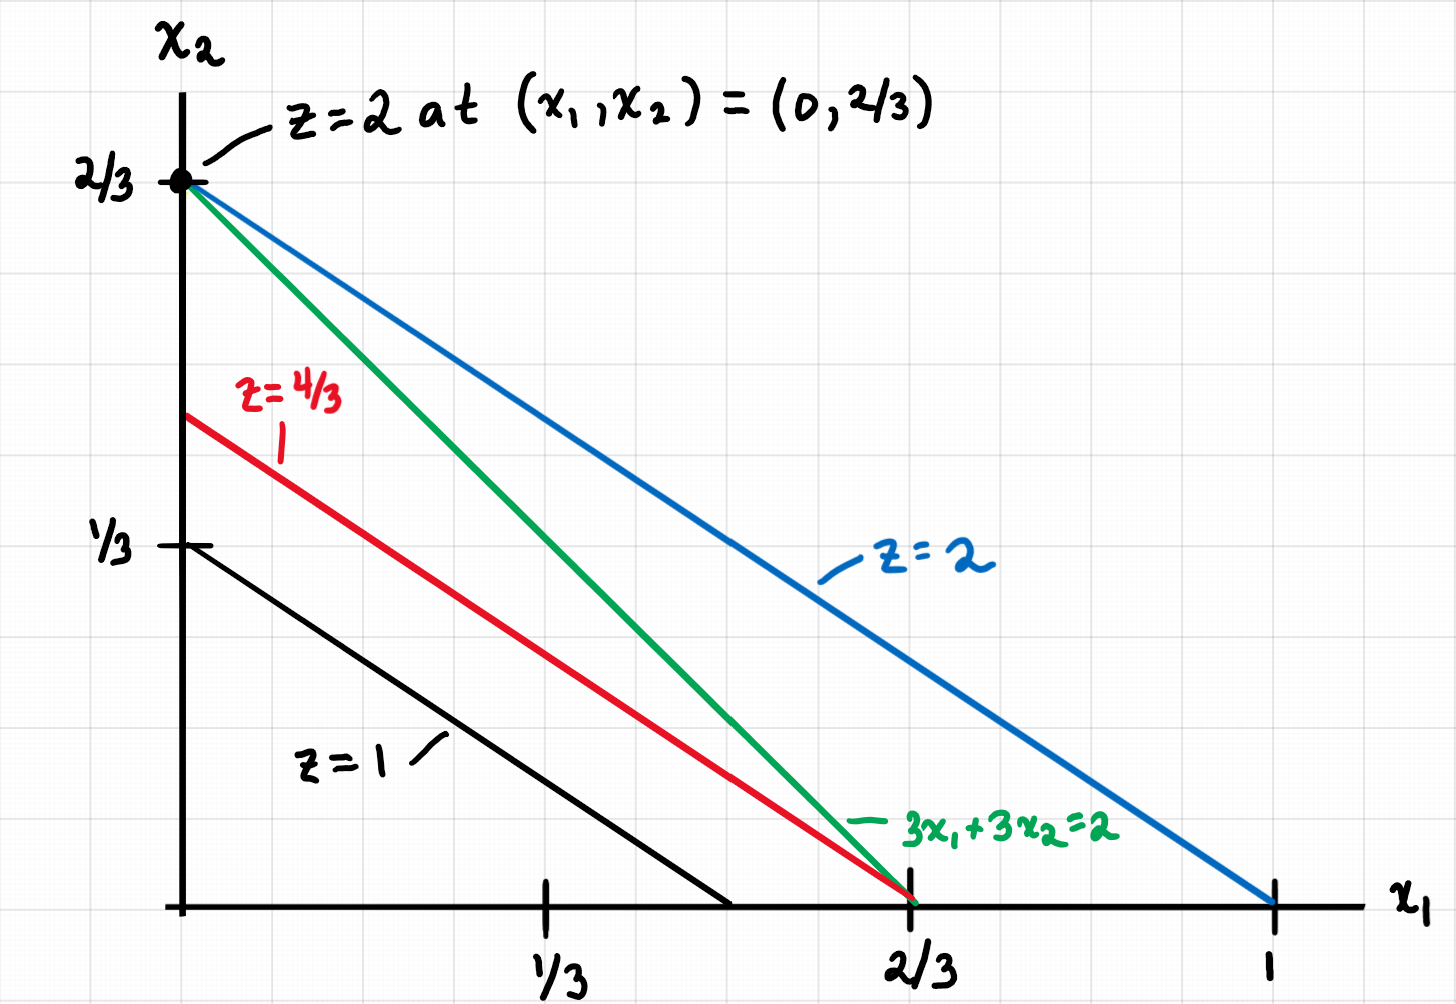
\includegraphics[width=0.65\linewidth]{Capture 2.png}
\end{figure}

\end{enumerate}

\end{document}